%%%%%%%%%%%%%%%%%%%%%%%%%%%%%%%%%%%%%%%%%%%%%%%%%%%%%%%%%%%%%%%%%%%%%%%%%%%%%%%%
% Social Network Analysis for Computer Scientists
% Course paper template (modified version of ACM Proceedings template)
% Frank W. Takes (ftakes@liacs.nl)
% http://liacs.leidenuniv.nl/~takesfw/SNACS
%%%%%%%%%%%%%%%%%%%%%%%%%%%%%%%%%%%%%%%%%%%%%%%%%%%%%%%%%%%%%%%%%%%%%%%%%%%%%%%%

% THIS IS SIGPROC-SP.TEX - VERSION 3.1
% WORKS WITH V3.2SP OF ACM_PROC_ARTICLE-SP.CLS
% APRIL 2009
%
% It is an example file showing how to use the 'acm_proc_article-sp.cls' V3.2SP
% LaTeX2e document class file for Conference Proceedings submissions.
% ----------------------------------------------------------------------------------------------------------------
% This .tex file (and associated .cls V3.2SP) *DOES NOT* produce:
%       1) The Permission Statement
%       2) The Conference (location) Info information
%       3) The Copyright Line with ACM data
%       4) Page numbering
% ---------------------------------------------------------------------------------------------------------------
% It is an example which *does* use the .bib file (from which the .bbl file
% is produced).
% REMEMBER HOWEVER: After having produced the .bbl file,
% and prior to final submission,
% you need to 'insert'  your .bbl file into your source .tex file so as to provide
% ONE 'self-contained' source file.
%
% For tracking purposes - this is V3.1SP - APRIL 2009

\documentclass{acm_proc_article-sp}

\usepackage{url}
\usepackage[utf8x]{inputenc}
\usepackage{tabulary}

\newtheorem{lem}{Lemma}
\newtheorem{thm}{Theorem}

\begin{document}

\title{Data-driven social influence maximization for modern social networks}
\subtitle{Social Network Analysis for Computer Scientists --- Course Project Paper}

\numberofauthors{2} %  in this sample file, there are a *total*
% of EIGHT authors. SIX appear on the 'first-page' (for formatting
% reasons) and the remaining two appear in the \additionalauthors section.
%
\author{
% You can go ahead and credit any number of authors here,
% e.g. one 'row of three' or two rows (consisting of one row of three
% and a second row of one, two or three).
%
% The command \alignauthor (no curly braces needed) should
% precede each author name, affiliation/snail-mail address and
% e-mail address. Additionally, tag each line of
% affiliation/address with \affaddr, and tag the
% e-mail address with \email.
%
% 1st. author
\alignauthor
	Steinar Bragi Sigurðarson\\
	\affaddr{LIACS, Leiden University}\\
	\email{s.b.sigurdarson@umail.leidenuniv.nl}
% 2nd. author
\alignauthor
	Xin Guo\\
	\affaddr{LIACS, Leiden University}\\
	\email{s1882201@umail.leidenuniv.nl}
}

\permission{This paper is the result of a student course project, and is based on methods and techniques suggested in \cite{goyal:datainfluence, kempe:maxspread, singer:winfriends,DBLP:journals/corr/HeK16}.  % NOTE for SNACS: replace these citations with the papers you studied!
Permission to make digital or hard copies of all or part of this work for personal or classroom use is granted without fee provided that copies are not made or distributed for profit or commercial advantage and that copies bear this notice on the first page. }
\conferenceinfo{SNACS '17}{Social Network Analysis for Computer Scientists, Master CS, Leiden University (\url{liacs.leidenuniv.nl/~takesfw/SNACS}).}

\date{}
% Just remember to make sure that the TOTAL number of authors
% is the number that will appear on the first page PLUS the
% number that will appear in the \additionalauthors section.

\maketitle
\begin{abstract}
Influence maximization is the problem of finding an optimal set of influencial nodes in a network to maximize the spread of information. Social networks have grown and evolved in recent years, and so have the methods of solving this problem. In this paper, we will discuss approaches from previous papers, while focusing on a promising data-based approach. We will compare the performance by applying it to multiple different networks and discuss the results of our experiments.
\end{abstract}

% A category with the (minimum) three required fields
\category{H.4}{Information Systems}{Social Networks}

\terms{Theory}

\keywords{Social Networks, Data Mining, Influence Spread, Credit Distribution} % NOT required for Proceedings

\section{Introduction}
Influence Maximization is a problem that has been studied thoroughly over the years and dates back further than our earliest online social networks. Ever since humans started connecting with each other through the Internet, there have been people who have been interested in the potential value of being able to reach and influence as many users in a network as possible with the least amount of effort, resources and complexity. During the early days of influence spread research, spread maximization was achieved by analyzing centrality measures in relatively small social graphs. Later, during the widespread adoption of online social networks the motivation for this started revolving around viral marketing, wanting to initiate and maximize the reach of word-of-mouth advertising campaigns. Since then, social networks have changed and grown tremendously as more and more people adopt these novel efficient means of communication. Recently it has become more apparent that entities might be using this type of knowledge to influence communities for other purposes than viral advertising. Foreign powers might want to affect outcomes of elections in other countries for economic or political gain by targeting users with tailored news articles in order to influence to tone of widespread debate and discussion. \textit{(There is evidence to suggest that this might have happened during the last presidential elections in the United States)}. Increasingly, the companies behind the social networks we use, are collecting an ever larger amount of behavioral information. This information can be used to predict the behaviour of nodes and target potential influential users with tailored content.

\subsection{The varying nature of social graphs}

Social networks vary in structure and have diffrent characteristics because they serve different purposes. The behaviour of users will vary accross networks. Many of us are regular users of multiple social networks. On Facebook, we might be discussing and chatting with a narrow group of reasonably close friends while we might choose to follow complete strangers and celebrities on Twitter based on their interests and opinions. The way we interact with people will vary in different contexts. The way this information is presented also affects our behavior. The algorithms that curate the news feeds of these various networks all have their own sets of specific characteristics. This affects what we can see, along with our options for reacting to the data we are presented with. We assume that these differences may affect the way information can spread. In this paper, we will describe and compare the spread of influence through different networks in order to find the most suitable structures for influence maximization.

\subsection{Using available data to predict\\ influenceability}
Social graphs are growing at such a rate, that the early methods of finding seed nodes are becoming increasingly unrealistic. They relied on computationally expensive probabilistic simulations to estimate the influence-ability of nodes in order to build sets of seed nodes. They ignore potential beneficial factors that could be considered when selecting nodes. Later studies introduced methods to exploit previous propagation traces to evaluate the influenceability of nodes, avoiding the need for guesswork and costly simulations.\cite{goyal:datainfluence} They distribute credit to potential influencers of nodes and give them a score, their probability of influence. These methods proved to be vastly superior, more efficient and scalable than previous techniques according to their experiments. Some of the most recent work, such as [Robust influence maximization, Xinran He, David Kempe 2016], suggested that we should consider even more diverse behavioural and environmental data to predict influence. We could find nodes to spread certain topics based on their interests, political leanings and opinions. In their paper they experimented with various data sets to try to identify a set of k nodes who are simultaneously influential for multiple functions or models.


\section{Related and previous work}

In all of the research we have studied, the optimization problems have been focused on finding an initial set of “seed” nodes which would maximize the influenceability through a network. \\

In 2003, a time before Facebook and Twitter, Kempe et al. \cite{kempe:maxspread}, suggested probabilistic simulation oriented approaches to select an initial set of seed nodes to maximize spread and cause a cascade effect through a network. They compared their novel techniques with older models and proved with various experiments that their methods outperform those which were based on classic graph measures such as degree centrality and distance centrality. Their focus was on Independent Cascade and Linear Threshold Models.In both, at a given time, each node can be either active or inactive. Each node's tendency to become active increases monotonically as more of its neighbors become active, and an active node never becomes inactive again. Time unfolds in discrete steps.

Yaron Singer \cite{singer:winfriends} focused on economic sides of the problem. He studied and proposed mechanisms to increase the influence-ability of users by compensating them financially, to create incentives and reward users for spreading information.

In 2016, Xinran He and Kempe \cite{DBLP:journals/corr/HeK16} proposed using multiple models simultaneously to predict influence spread. They argued that what defines a “social tie” can in many cases be fuzzy and unclear. They also argued that human behaviour is typically influenced by many environmental variables, such as interests and opinions matching a particular topic to be spread. Based on the assumption that multiple factors can affect the influence-ability of nodes, they designed an algorithm that finds nodes that are simultaneously influential for multiple functions. Their experiments showed that combining models improved the accuracy of spread prediction. Their research was funded by the U.S. Defence Advanced Research Projects Agency, (DARPA) under Social Media in Strategic Communication (SMISC) program.


Goyal et Al \cite{goyal:datainfluence} proposed a novel approach in 2012. They argued that using probabilistic Monte Carlo simulations to scan a network for potential seed nodes isn't scalable for real world large networks. Their novel approach was to scan and exploit an Action Log, a log containing previous propagation traces and use those to distribute credit (influence probability score) throughout the network, avoiding the need for costly simulations. This is the approach we will be focusing on in this paper.


\section{Problem Statement}

\begin{figure}
	\centering
	\begin{tabulary}{\linewidth}{|l|L|}
			\hline
			$G$ & A Directed Graph, $G = (V,E)$ \\\hline
			$V$ & Nodes, $V = \{u,v,w,x,...\}$ \\\hline
			$E$ & Edges, $E = \{(u, v),(w, v),(v,w),...\}$ \\\hline
			$S$ & Seed set of influencial nodes \\\hline
			$k$ & Number of nodes in a seed set \\\hline
	\end{tabulary}
	\caption{Graph Notation}
	\label{general-notation}
\end{figure}

Our main goal, like others before us is to find a $k$ set of seed nodes $S$ that maximizes influence spread through a social network. The credit distribution model from Goyal et al has been proven to be a more scalable, efficient and accurate model than IC and LT discussed in \cite{kempe:maxspread}. Our contribution will be to compare the performance of the credit distribution model using multiple social graphs with varying structure and nature. The purpose is to gain insight and describe the properties of an optimal dataset for which this approach is the most suitable.

\subsection{Credit distribution}

The process starts with the (unweighted) social graph and a log of past action propagations that say when each user performed an action. If we take a social music streaming service as an example, the log might contain recorded actions such as listening to a song. If a user listens to a song, and his friend later listens to the same song, we can consider the action to have propagated from the first user to his friend. The log is used to estimate influence probabilities among the nodes. This produces the directed edge-weighted graph which is then given as input to the greedy algorithm which produces the seed set. They look at potential influencers for actions performed by each node and distribute credit evenly between nodes who previously performed the same action. Nodes can influence other nodes indirectly. The total propagation score for a pair of nodes is the sum of direct and indirect influence scores.

\section{Suggested Approaches}

We want to study the structure of various datasets to find out which characteristics are important for the CD model to be successful. We will compare the performance over multiple datasets and try to describe the attributes required for successful CD based influence spread. The datasets we are studying require different preprocessing approaches. One of our main challenges is the splitting of action logs $\mathbb{L}$ into meaningful training and test sets, in order to measure our accuracy in a meaningful manner. For credit distribution and spread prediction we are using the software provided in \cite{goyal:datainfluence} along with our own custom preprocessing scripts. After preprocessing, we use the previously mentioned software to select seed nodes, predict spread and compare with actual spread.

The seed selection process is described in detail in \cite{goyal:datainfluence}. We will briefly summarize some of the the most relevant points here. For each action performed by a node \textit{u} in our action log $\mathbb{L}$, the algorithm distributes credit evenly between direct neighbours \textit{w} of \textit{u}, if they performed the same action before \textit{u}. It also distributes credit backwards to all \textit{predecessors} of \textit{u} in \textit{G} who also performed the same action. To calculate the final score for a pair they use the formula in figure ~\ref{CD-formula}. See notation in table ~\ref{notation2}.

\begin{figure}[h]
	\begin{tabulary}{\linewidth}{|l|L|}
			\hline
			$\mathbb{L}$ & Action log \\\hline
			$A_u$ & Total number of actions performed by node $u$ \\\hline
			$\gamma_{v,u}(a)$ & Direct influence credit given to $v$ for influencing $u$ for action a \\\hline
			$\Gamma_{v,u}(a)$ & Total credit given to $v$ for influencing $u$ for action $a$ \\\hline
			$\kappa_{v,u}$ & Total credit given to v for influencing u for all actions \\\hline
	\end{tabulary}
	\caption{CD Notation from Goyal et al. \cite{goyal:datainfluence}}
	\label{notation2}
\end{figure}


\begin{figure}[h]
	\begin{equation}
		\Gamma_{v,u}(a) = \displaystyle\sum_{w \in N_{in}(u,a)} \Gamma_{v,w}(a) \cdot \gamma_{w,u}(a)
	\end{equation}
	\label{CD-formula}
\end{figure}

While scanning the graphs and action logs, the algorithms add nodes to the seed set $S$ if they improve the total influence spread score by computing the marginal gain for each node addition. If there is no gain to adding a seed node to the set, it is discarded.

\subsection*{Aggregating over all actions and all nodes}

Next, Goyal et al. described how they would aggregate the influence credit over the whole action log $\mathbb{L}$. Consider two nodes $v$ and $u$: the total influence credit given to $v$ by $u$ for all actions in $A$, is simply obtained by taking the total credit over all actions and normalizing it by the number of actions performed by $u$ (denoted $A_u$). This is justified by the fact that credits are assigned by $u$ backward to its potential influencers. In their paper \cite{goyal:datainfluence}, Goyal et al. defined the following formulas:

\begin{equation}
	\kappa_{v,u} = \frac{1}{A_u} \displaystyle\sum_{a \in A} \Gamma_{u,v}(a)
\end{equation}

\noindent This denotes the average credit given to $v$ for influencing $u$, over all actions that $u$ performs. Similarly, for the case of a set of nodes $S \subseteq V$ , they define the total influence credit for all the actions in $A$ as:
\begin{equation}
		\kappa_{S,u} = \frac{1}{A_u} \displaystyle\sum_{a \in A} \Gamma_{S,v}(a)
\end{equation}

\noindent Finally, they define the influence spread $\sigma_m{cd}(S)$ as the total influence credit given to $S$ from the whole social network:
\begin{equation}
	\sigma_{cd}(S) = \displaystyle\sum_{u\in V} \kappa_{S,u} = \displaystyle\sum_{u\in V} \frac{1}{A_u} \displaystyle\sum_{a \in A} \Gamma_{S,v}(a)
\end{equation}

This is the objective function that the algorithms in \cite{goyal:datainfluence} attempt to maximize. We will be comparing the seed sets and the influence credits obtained by various datasets, described in the next chapter.



\section{Datasets}

In order to find out which types of graphs are the most suitable for the credit distribution model, we need to study the characteristics of various social graphs and find links between their structure and the achieved spread for our seed sets of nodes. Our requirements are that each social graph needs to have an accompanying action log $\mathbb{L}$ containing previous propagation traces. We compared 4 datasets which will be described below.

\textbf{Flickr} \cite{data:flickr} is a social photo sharing platform. It's underlying social network is an directed graph. Users can follow each other and get notified of their friends submissions and activity. We used a subset of Flickr friendships as our social graph. Each action in the accompanying action log represents a user marking a photo as a favourite. We studied the propagation of this action accross friendships in the newtork. \cite{data:flickr-paper}

\textbf{Flixster} \cite{data:flixster} is an online social movie database. Flixter's action log consists of movie ratings. We looked at the propagations of movie ratings throughout Flixter's friendship network. \cite{data:flixsterpaper}

\textbf{Digg} \cite{data:digg-friends,data:digg-votes,data:digg} Digg is social news aggregator. In it's previous form, users could "digg" or "bury" stories, similar to the upvoting and downvoting functionality on reddit. Digg had a global front page, which would look the same for every user at every given time. It isn't individually tailored like Twitter's front page. The front page featured stories which had high "digg" scores. In 2005, Digg added a friend list feature, which allowed users to follow each other's activity by clicking on a \textit{Friends Activity} tab. The frienship graph is directed, like Twitter, meaning that listing someone as a friend isn't neccesarily mutual. When user A lists user B as a friend, A can watch the activities of B but not vice versa. If B votes on a story, this action becomes visible to A. Our action log contains votes on stories and we will measure how they propagate. \cite{DBLP:journals/corr/abs-1202-3162}

\textbf{Twitter} \cite{data:twitter} is a directed social network. It has gained temendous popularity and widespread adoption in recent years for its ease of use. Users follow other users and can very easily "retweet" posts with a single click. This feature makes it easy for users to share and spread content with their followers. It simplifies the process of influencing followers and we suspect it might have a big impact on the performance of credit distribution influence maximization. The front page of Twitter is generated by various algorithms which curate a news feed of potentially interesting tweets for each user based on who they follow and have interacted with in the past. Tweets can contain \textit{\#hashtags}, which represent certain topics. An example of a notable hashtag is \textit{\#metoo}, which has spread throughout the whole world in recent weeks. The hashtag and the women behind it were featured as the latest Time Magazine Person of the Year. Our action log for twitter is based on URLs that have propagated through retweets.
 \cite{DBLP:journals/corr/abs-1202-3162}

\subsection*{Preprocess}
We convert each raw friendship network data to a new form containing three columns: use\_id, follower\_id and timestamp of becoming friend. Here the time of becoming friend is set as zero because we only focus on the static friendship network which don't grow any more as time unfolds. Then, each graph is pruned as simple graph which do not contain self loop and multiple edges. Finally, the largest weakly connected component detected from the directed graph is saved and used as one of input of influence spread software.

Also, we convert each action log, which is crawled from associated websites during a specific time period, to the form containing three columns: user\_id, action\_id and timestamp of performing this action. Here \textit{action} has different meaning in each specific dataset. In Flickr, action\_id refers to photo\_id marked as favorite, rated movie\_id in Flixster, voted story\_id in Digg , URL\_id contained in retweet in Twitter, respectively. We group the action log by action\_id and sort timestamp chronologically. Finally, we split action log into training set (80\%) and testing set (20\%). The statistics of our datasets shows in Table \ref{table1}.

 
\begin{table}[]
	\centering
	\caption{Statistics of Datasets}
	\label{table1}
	\begin{tabular}{|l|l|l|l|l|}
		\hline
		& Flixster  & Flickr    & Digg      & Twitter    \\ \hline
		\#Nodes         & 1,049,512 & 850,808   & 154,514   & 699,985    \\ \hline
		\#Dir.Edges     & 7,058,819 & 331,4002  & 886,335   & 36,743,448 \\ \hline
		\#action id     & 48,794    & 909,197   & 3,553     & 66,059     \\ \hline
		\#tuples in log & 8,196,077 & 1,379,598 & 3,018,197 & 1,342,312  \\ \hline
	\end{tabular}
\end{table}


\section{Experiments and results}
\textbf{TODO: Compare the performance of the credit distribution model with the different datasets}

\subsection*{Spread Achieved}
In this experiments, we compare the influence spread achieved by the seed sets obtained from CD model, among the four real social networks along with user activities logs. Considering the differences among those datasets in nature, we first compare Flixster and Flickr and then add Digg and Twitter.

First, we'll compare Flickr and Flixster in  ~\ref{spread2}. As we can see from the Flickr results, we barely managed any significant spread. The achieved number of activated nodes is about the same as the number of nodes in our seed set. This indicates that the action of marking a photo as a favourite does not propagate to friends. This might be due to the user interface. Photos favorited by friends do not become more prominent in the news feed, so these actions go unnoticed and do not affect the behaviour of friends. In the flixter data, each rating propagated to around 1 friend on average, which results in a score approximately two times higher than Flickr's.

\begin{figure}[h]
	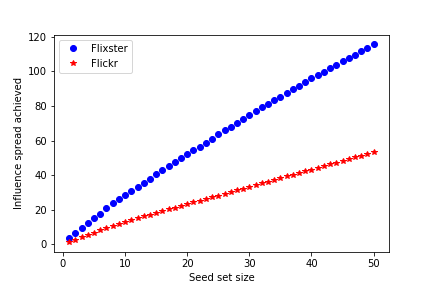
\includegraphics[width=\linewidth]{spread2.png}
	\centering
	\label{spread2}
	\caption{Achieved spread by seed sets under CD model on Flickr \& Flixster}
\end{figure}

In ~\ref{spread3} we see the achieved spread of Digg compared to Flickr and Flixster. We can clearly see that action propagations are much stronger in the Digg network compared to the other two.

\begin{figure}[h]
	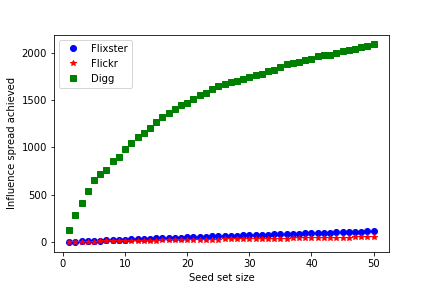
\includegraphics[width=\linewidth]{spread3.png}
	\centering
	\label{spread3}
    \caption{Achieved spread by seed sets under CD model on Digg, Flickr \& Flixster}
\end{figure}

While scanning the Twitter network, we saw noticable jumps in the overall influence spread score along the way. These jumps denote highly influencial nodes being detected, pulling the overall score up significantly. We also notice that Twitter is an even better fit than Digg for influence maximization. We suspect this might be due to the design of the frontpage. The primary purpose of Twitter's social network is to connect with and spread information to followers. The website revolves around the activity of posting bite size pieces of information and resharing interesting tweets.

\begin{figure}[h]
	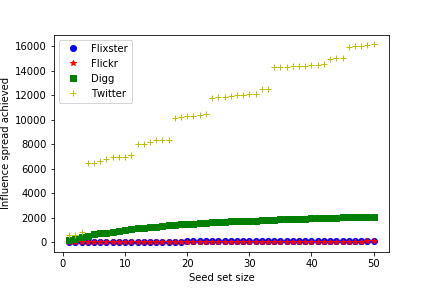
\includegraphics[width=\linewidth]{spread4.png}
	\centering
	\label{spreadall}
    \caption{Achieved spread of all 4 networks}
\end{figure}

\subsection*{Accuracy of Spread Prediction}

Figure \ref{accuracy} shows an intuitive difference among four real social networks along with user action logs. On one hand, actual spread under both Digg and Twitter datasets is further and wider than that under Fixster and Flickr. On the other hands, the relative prediction error of CD model under Digg is obviously less than those under the other three datasets.

\begin{figure}[h]
	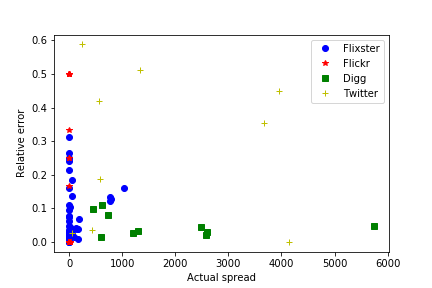
\includegraphics[width=\linewidth]{accuracy.png}
	\centering
	\label{accuracy}
    \caption{Prediction accuracy on all 4 datasets}
\end{figure}


\section{Conclusions}

%\end{document}  % This is where a 'short' article might terminate

%
% The following two commands are all you need in the
% initial runs of your .tex file to
% produce the bibliography for the citations in your paper.
\bibliographystyle{abbrv}
\bibliography{influence.bib}  % sigproc.bib is the name of the Bibliography in this case
% You must have a proper ".bib" file
%  and remember to run:
% latex bibtex latex latex
% to resolve all references
%
% ACM needs 'a single self-contained file'!

\balancecolumns
% That's all folks!
\end{document}
